\markboth{GUI tools}{GUI tools}
\section{GUI tools}
For a quick and easy set-up of a battery model, two GUI tools were created as part of this package. Since both tools are based on \java\ Swing, a \java\ virtual machine (JVM) must be installed for the GUI tools to function. Normally, \matlab\ comes pre-bundled with a JVM. However, in the rare cases in which this is not the case, an error message is printed to the command window.

\subsection{Battery Pack Designer}
The Battery Pack Designer is a GUI that enables the creation of a \mcode{batteryPack} object. It can be started by typing
\begin{lstlisting}
batteryPack.GUI
\end{lstlisting}
into the command window. Figure~\ref{fig:Designer} shows a screenshot of the tool in Windows. Usage of the tool should be self-explanatory. Detailed information is provided using tool tips, which appear when hovering over GUI element (i.e. button or text field) with the mouse. When the model is fully configured, a \mcode{batteryPack} object can be created and sent to the workspace. The Battery Pack Designer provides a comfortable way to create models for users who are new to the package. It can be practicable for the purpose of getting to know the model and it's interface. \\
However, it is not recommended to save the created objects in MAT files for later use in simulations. Object links within the model (i.e. the link between the age model and the pack; see section~\ref{sec:ageModel}) are broken upon saving, which may result in unexpected behaviour of the loaded objects. 
\begin{figure}[b!]
	\captionsetup{type=figure}
	\centering
	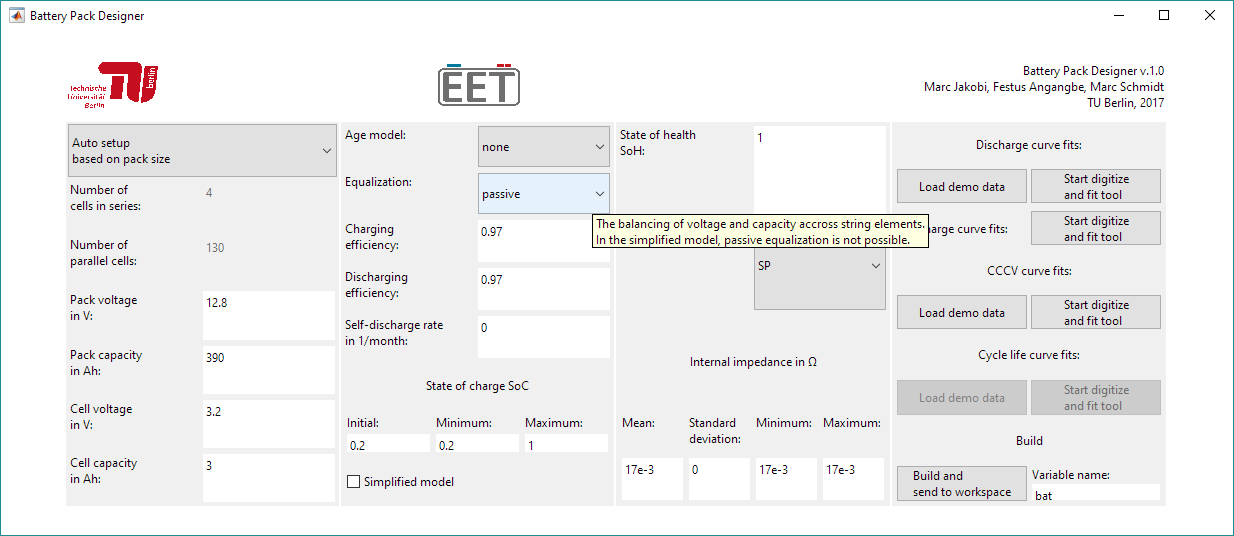
\includegraphics[width=\textwidth]{Designer.png}
	\caption[Screenshot of the Battery Pack Designer in Windows]{Screenshot of the Battery Pack Designer in Windows.}
	\label{fig:Designer}
\end{figure}
Furthermore, if multiple battery cells hold references to a single \mcode{dischargeCurves} object (see section~\ref{sec:dischargeCurvesMain}), the object is deep-copied across all of the cells, potentially resulting in large amounts of data\footnote{This can be fixed by re-adding the \mcode{dischargeCurves} using the \mcode{addcurves()} method after loading.}. The creation of deep-copies upon saving could also lead to memory leaks. Due to this behaviour, it is recommended to initialize the \mcode{batteryPack} at runtime, before the simulation (see section~\ref{sec:batteryPackConstructor}).